%%%%%%%%%%%%%%%%%%%%%%%%%%%%%%%%%%%%%%%%%%%%%%%%%%%%%%%%%%%%%%%
%\subsection{Task 1}
%\label{sub:task1}
%%%%%%%%%%%%%%%%%%%%%%%%%%%%%%%%%%%%%%%%%%%%%%%%%%%%%%%%%%%%%%%

Task 1 comprises the generation of synthetic models (conforming the movie database metamodel~\cite{imdbcase}) from an input parameter $N \geq 0$. We first present an e-Motions solution and then a Maude solution. 


%%%%%%%%%%%%%%%%%%%%%%%%%%%%%%%%%%%%%%%%%%%%%%%%%%%%%%%%%%%%%%%
\subsubsection{e-Motions-based solution.}

Following an e-Motions based approach, we define the abstract and concrete syntax and the behavior of our so-called \textit{Task 1 DSL}. Taking a parameter $N$ as input model, \textit{Task 1 DSL} generates a model containing synthetic data.

As it has been introduced in Section~\ref{sub:emotions}, the abstract syntax of a DSL is given in e-Motions by means of an Ecore metamodel. Since we model the solution of the task as a model that evolves until reaching its final solution, we take as metamodel the one provided beforehand in~\cite{imdbsources}, which we call \textit{Movies MM}, extended with a \code{Parameter} concept. This results in a so-called \textit{Movies* MM}. The class \code{Parameter} has two integer attributes, namely \code{nP} and \code{nN}, which represent positive graphs and negative graphs, respectively, for the generation following Henshin graphs~\cite{Henshin:10}.

For the concrete syntax, Figure~\ref{fig:concreteSyntax} shows how an image has been attached to each concept modeled in the Movies* MM. 

The behavior of this \textit{Task 1 DSL} is then given by means of two in-place transformation rules: \code{createPositive} and \code{createNegative}. Figure~\ref{fig:createPositive} shows the \code{createPositive} rule, which takes an object \code{p} of type \textit{Parameter}, with \textit{nP} attribute greater or equal than $0$, and produces synthetic data conforming to the Henshing rules~\cite{Henshin:10}. Figure~\ref{fig:createNegative} shows the \code{createNegative} rule, which is analogously defined.

\begin{figure}[tb]
  \subfloat[Actor.\label{fig:actor}]{
    \makebox[60px][c]{
\includegraphics[scale=1]{imgs/actor}}
  }
  \hfill
  \subfloat[Actress.\label{fig:actress}]{
    \makebox[60px][c]{
\includegraphics[scale=1]{imgs/actress}}
  }
  \hfill
  \subfloat[Movie.\label{fig:movie}]{
    \makebox[60px][c]{
\includegraphics[scale=1]{imgs/movie}}
  }
  \hfill
  \subfloat[Couple.\label{fig:couple}]{
    \makebox[60px][c]{
\includegraphics[scale=1]{imgs/couple}}
  }
  \hfill
  \subfloat[Parameter.\label{fig:parameter}]{
    \makebox[60px][c]{
\includegraphics[scale=1]{imgs/parameter}}
  }
  \caption{Concrete syntax for \textit{Movies* MM}.}
  \label{fig:concreteSyntax}
\end{figure}

\begin{figure}
  \subfloat[The \code{createPositive} rule.\label{fig:createPositive}]{%
    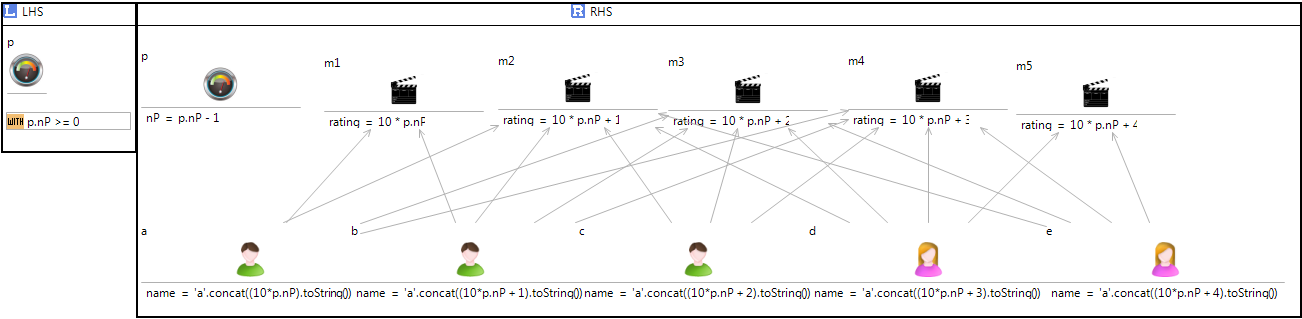
\includegraphics[width=\textheight, angle=90]{imgs/createPositiveRule}
  }
  \hfill
%  \subfloat[Rules' headers.]{
%    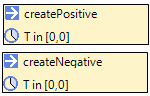
\includegraphics[width=0.2\textwidth]{imgs/headersCreate}
%  }
%  \hfill
  \subfloat[The \code{negativePositive} rule.\label{fig:createNegative}]{%
    \ \ \ \ 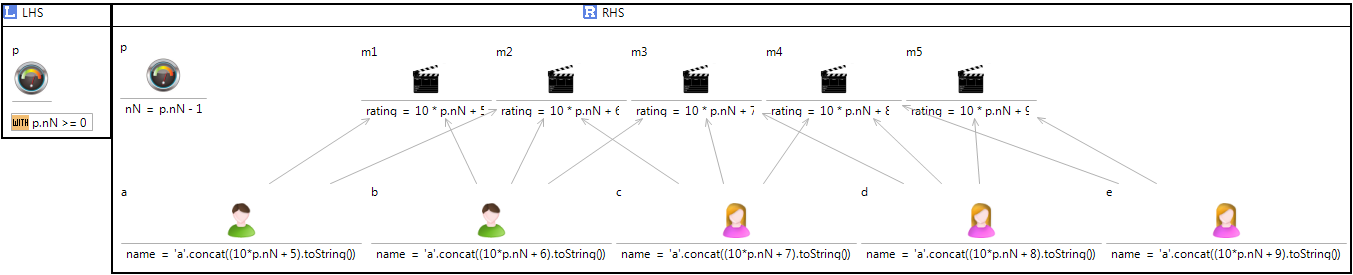
\includegraphics[width=\textheight, angle=90]{imgs/createNegativeRule}\ \ \ \ 
  }
  \caption{Task 1 rules. \label{fig:task1}}
\end{figure}

Once the syntax and the behavior of the system has been coded, the user may specify a model, which conforms to \textit{Movies* MM}, containing an object \code{Parameter} with its two attributes \code{nP} and \code{nN} properly set. This model is used as initial model of the execution.

Please, note that this solution is really close to the problem specification in~\cite{imdbcase}. Figure~\ref{fig:task1} and~\cite[Figure~2]{imdbcase}, specifying the data generation, are almost the same. This demonstrates how close the solution by e-Motions is to the problem domain, and how convenient its graphical facilities are.

\subsubsection{Maude version.}
Our Maude-based solution for Task 1 consists of an object-based Maude specification, consisting of two modules: the \code{MOVIES@MM} module defining the classes structure, and the \code{TASK1} module defining the rewrite rules to calculate the solution. As in the e-Motions solution, we have two rewrite rules: \code{createPositive} and \code{createNegative}. Listing \ref{lst:createPositive} shows the \code{createPositive} Maude rule, that takes the \code{createPositive(s(N:Nat))} message and a \code{freshOid} auxiliary message---used to create new object identifiers---and returns such a object configuration conforming the Henshin specification~\cite{imdbcase}. A similar rule generates the negative cases. Please notice that the Maude version is very much like the e-Motions version. In fact, the former is almost the textual version of the latter. 

\begin{lstlisting}[caption=\code{createPositive} Maude rule., label=lst:createPositive]
rl [createPositive] :
  createPositive(s(N))
  freshOid(N')
=>
  createPositive(N)
  < N'     : Movie | rating: (10.0 * float(N)) >
  < N' + 1 : Movie | rating: (10.0 * float(N) + 1.0) >
  < N' + 2 : Movie | rating: (10.0 * float(N) + 2.0) >
  < N' + 3 : Movie | rating: (10.0 * float(N) + 3.0) >
  < N' + 4 : Movie | rating: (10.0 * float(N) + 4.0) >
  
  < N' + 5 : Actor | name: ("a" + string(10 * N, 10)),
                   movies: (N', N' + 1, N' + 2, N' + 3) >
  < N' + 6 : Actor | name: ("a" + string(10 * N + 1, 10)),
                   movies: (N', N' + 1, N' + 2) >
  < N' + 7 : Actor | name: ("a" + string(10 * N + 2, 10)),
                   movies: (N' + 1, N' + 2, N' + 3) >
  < N' + 8 : Actress | name: ("a" + string(10 * N + 3, 10)),
                   movies: (N' + 1, N' + 2, N' + 3, N' + 4) >
  < N' + 9 : Actress | name: ("a" + string(10 * N + 4, 10)),
                   movies: (N' + 1, N' + 2, N' + 3, N' + 4) >
  freshOid(N' + 10) .
\end{lstlisting}

\subsubsection{Execution performance for both solutions.}

Table \ref{table:task1} shows the number of rewrites and execution times for both solutions. As explained above, the the execution times for the Maude specification obtained from the e-Motions definition grows very quickly. Notice that, although the number of rewrites grows linearly with respect to $N$, the time is exponential due to the infrastructure to deal with all the extra features in e-Motions. However, notice how the number of rewrites for the Maude solution grows linearly as well, but in this case the execution times grows more slowly, being able to handle problems of much bigger sizes.

\begin{table*}[tb]
\renewcommand{\tabcolsep}{6pt}
\renewcommand{\arraystretch}{1.2}
    \centering
	\begin{tabular}[tb]{r|r|r|r|r|}
%	\hline
	    & \multicolumn{2}{|c|}{e-Motions} & \multicolumn{2}{|c|}{Maude} \\
	\hline
	$N$ & Time (s) & \# Rewrites & Time (s) & \# Rewrites \\
	\hline
<<<<<<< HEAD
	1    &       &           & 0.0 &       67 \\
	2    &   0.0 &     4,910 & 0.0 &      133 \\ 
	10   &   0.0 &    24,334 & 0.0 &      661 \\
	20   &   0.0 &    48,614 & 0.0 &     1321 \\
	100  &   0.6 &   242,854 & 0.0 &     6601 \\
	1000 &  55.7 & 2,428,054 & 1.7 &  66,001 \\
	2000 & 395.0 & 4,856,054 & 11.8 & 132,001 \\
	3000 &       &           & 31.5 & 198,001 \\
	4000 &       &           & 40.8 & 264,001 \\
	5000 &       &           & 65.8 & 330,001 \\
	6000 &       &           & 96.8 & 396,001 \\
	7000 &       &           & 133.4 & 462,001 \\
	8000 &       &           & 175.8 & 528,001 \\
	9000 &       &           & 224.5 & 594,001 \\
  10000 &      &           & 227.9 & 660,001 \\
  11000 &      &           & 337.4 & 726,001 \\
	\hline 
=======
	1    &       &           & 0.0 &       68 \\
	2    &   0.0 &     4,910 && \\
	10   &   0.0 &    24,334 && \\
	20   &   0.0 &    48,614 && \\
	100  &   0.6 &   242,854 && \\
	1000 &  55.7 & 2,428,054 &   1.9 &  67,001 \\
	2000 & 395.0 & 4,856,054 &  12.7 & 134,001 \\
	3000 &       &           &  33.9 & 201,001 \\
	4000 &       &           &  64.1 & 268,001 \\
	5000 &       &           & 104.4 & 335,001 \\
	6000 &       &           & 109.6 & 402,001 \\
	7000 &       &           & 144.5 & 469,001 \\
%	\hline 
>>>>>>> 25376075b0d7a172a90b85b7d3c4fda7b15ed802
	\end{tabular}
	\vspace{.5cm}
	\caption{Times for the e-Motions and Maude solutions to Task 1}
	\label{table:task1}
\end{table*}

\subsubsection{On the correctness of the transformation}

Maude provides a whole formal environment where we can perform proofs of correctness of our solution. In addition to tools to verify the termination, confluence, etc. of our rewrite systems, Maude provides a reachability analysis tool and a model checker, which are particularly attractive for performing checks on the correctness of systems. Let us consider here the Maude \code{search} command, which allows us to explore the whole reachable state space, or up to a given depth, looking for states satisfying a given condition. 

For instance, following the results given in~\cite{imdbcase}, for some $N$, the above rules \code{createPositive} and \code{createNegative} create $20N$ objects, specifically, $10N$ movies, $5N$ actresses, and $5N$ actors. We could check that the solution found satisfies this condition, but we can do something more interesting by checking that no final reachable state fails to satisfy it. Of course, if the rewrite system is confluent and terminating the solution would be unique. 

Given the \code{numOfMovies} operation, which takes an object configuration as input and returns the number of movies in it, we may look for those final states in which the number of movies will be different than $10N$ (being N the parameter of the operation \code{createExample}):
\begin{verbatim}
  search createPositive(8) createNegative(8) freshOid(0) 
    =>! C:Configuration
    such that numOfMovies(C:Configuration) =/= 10 * 8 .
\end{verbatim}

The arrow \code{=>!} means that it search for final states, that is, states that cannot be further rewritten, starting from the given initial configuration, that satisfy the given condition. Maude returns no solution for the above code, that means all final states reached have exactly 10 movies:
\begin{verbatim}
  No solution.
\end{verbatim}
%  states: 5  rewrites: 180 in 0ms cpu (0ms real)


%\begin{table*}
%\renewcommand{\tabcolsep}{6pt}
%\renewcommand{\arraystretch}{1.2}
%	\caption{e-Motions times for Task 1.}
%	\label{table:emotionstask1}
%\centering
%	\begin{tabular}[tb]{r|r|r|}
%	$N$ & Time (s) & \# Rewrites \\
%	\hline
%	2 & 0.0 & 4,910 \\
%	10 & 0.0 & 24,334 \\
%	20 & 0.0 & 48,614 \\
%	100 & 0.6 & 242,854 \\
%	1000 & 55.7 & 2,428,054 \\
%	2000 & 395.0 & 4,856,054 \\
%	\hline 
%	\end{tabular}
%	\vspace{1cm}
%\end{table*}
%
%\begin{table}
%  \begin{center}
%	\begin{tabular}{r r r}
%	$N$ & Time (s) & \# Rewrites \\
%	\hline
%	1 & 0.0 & 68 \\
%	1000 & 1.9 & 67,001 \\
%	2000 & 12.7 & 134,001 \\
%	3000 & 33.9 & 201,001 \\
%	4000 & 64.1 & 268,001 \\
%	5000 & 104.4 & 335,001 \\
%	6000 & 109.6 & 402,001 \\
%	7000 & 144.5 & 469,001 \\
%	\hline \\
%	\end{tabular}
%	\caption{Maude times for Task 1.}\label{table:maudetask1}
%	\end{center}
%\end{table}
%
%
%
